\section{Spin precession}
\subsection{Set-up and procedure}
\begin{figure}
\centering
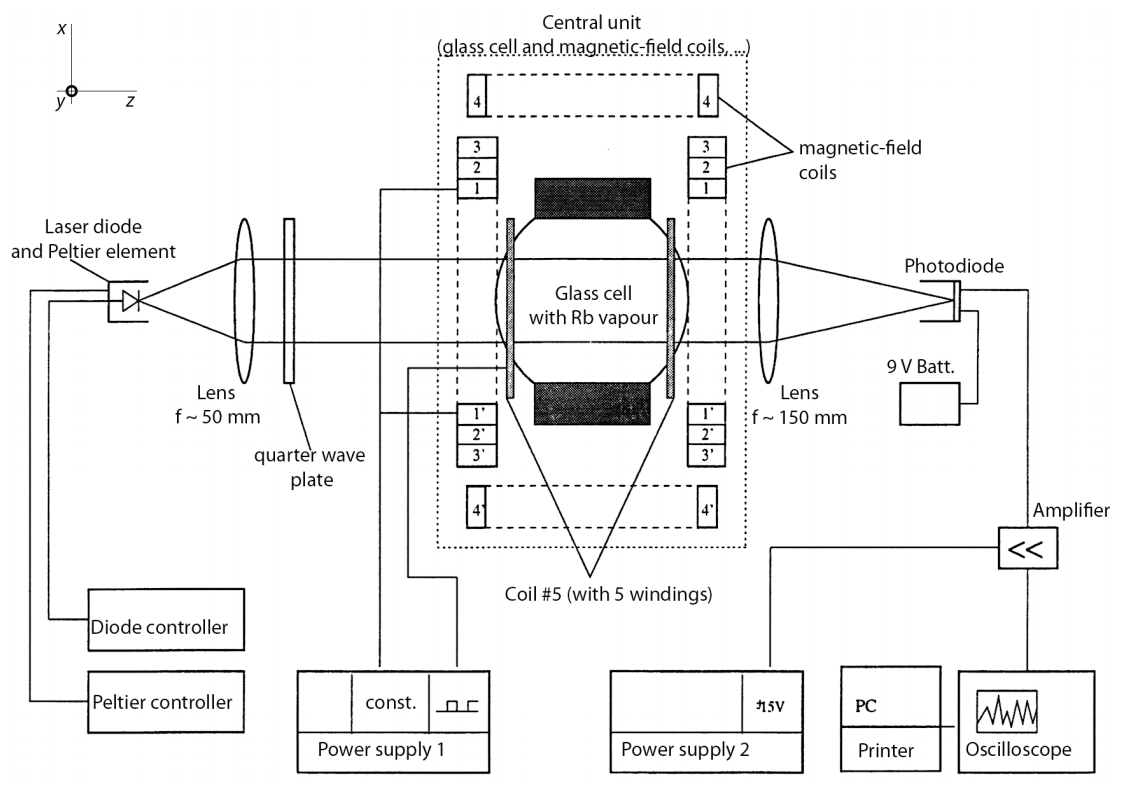
\includegraphics[width=1.0\linewidth]{graphics/spinprecessionsetup}
\caption[Spin precession set-up]{Experimental set-up for the spin precession measurements. \cite{anleitung}}
\label{fig:spinprecessionsetup}
\end{figure}
As before, only a quarter wave plate and the glass cell are placed in the beam. For the spin precession, the horizontal field as it was calculated in the double resonance section is compensated with a current in coil 1. A rectangular signal is given onto coil 5 so that the horizontal component of the magnetic field is compensated regularly. The spin precedes around the remaining vertical component, which can be varied by currents in coil 4. Measurements of the precession are then taken for a range of currents in coil 4.\\

Upon initial measurements, where both horizontal and vertical component were compensated as per the results from the double resonance section, it became clear that there was still a magnetic field, since precession could still be observed. As mentioned before, the table is not aligned with the horizontal component of the earths' magnetic field. Thus, the table was rotated until a minimal precession frequency was found. The degree by which the table was turned was $\phi=\unit{(7\pm2)}{\degree}$ and measurements were then taken as described above.

\subsection{Data analysis}
\begin{figure}
	\centering
	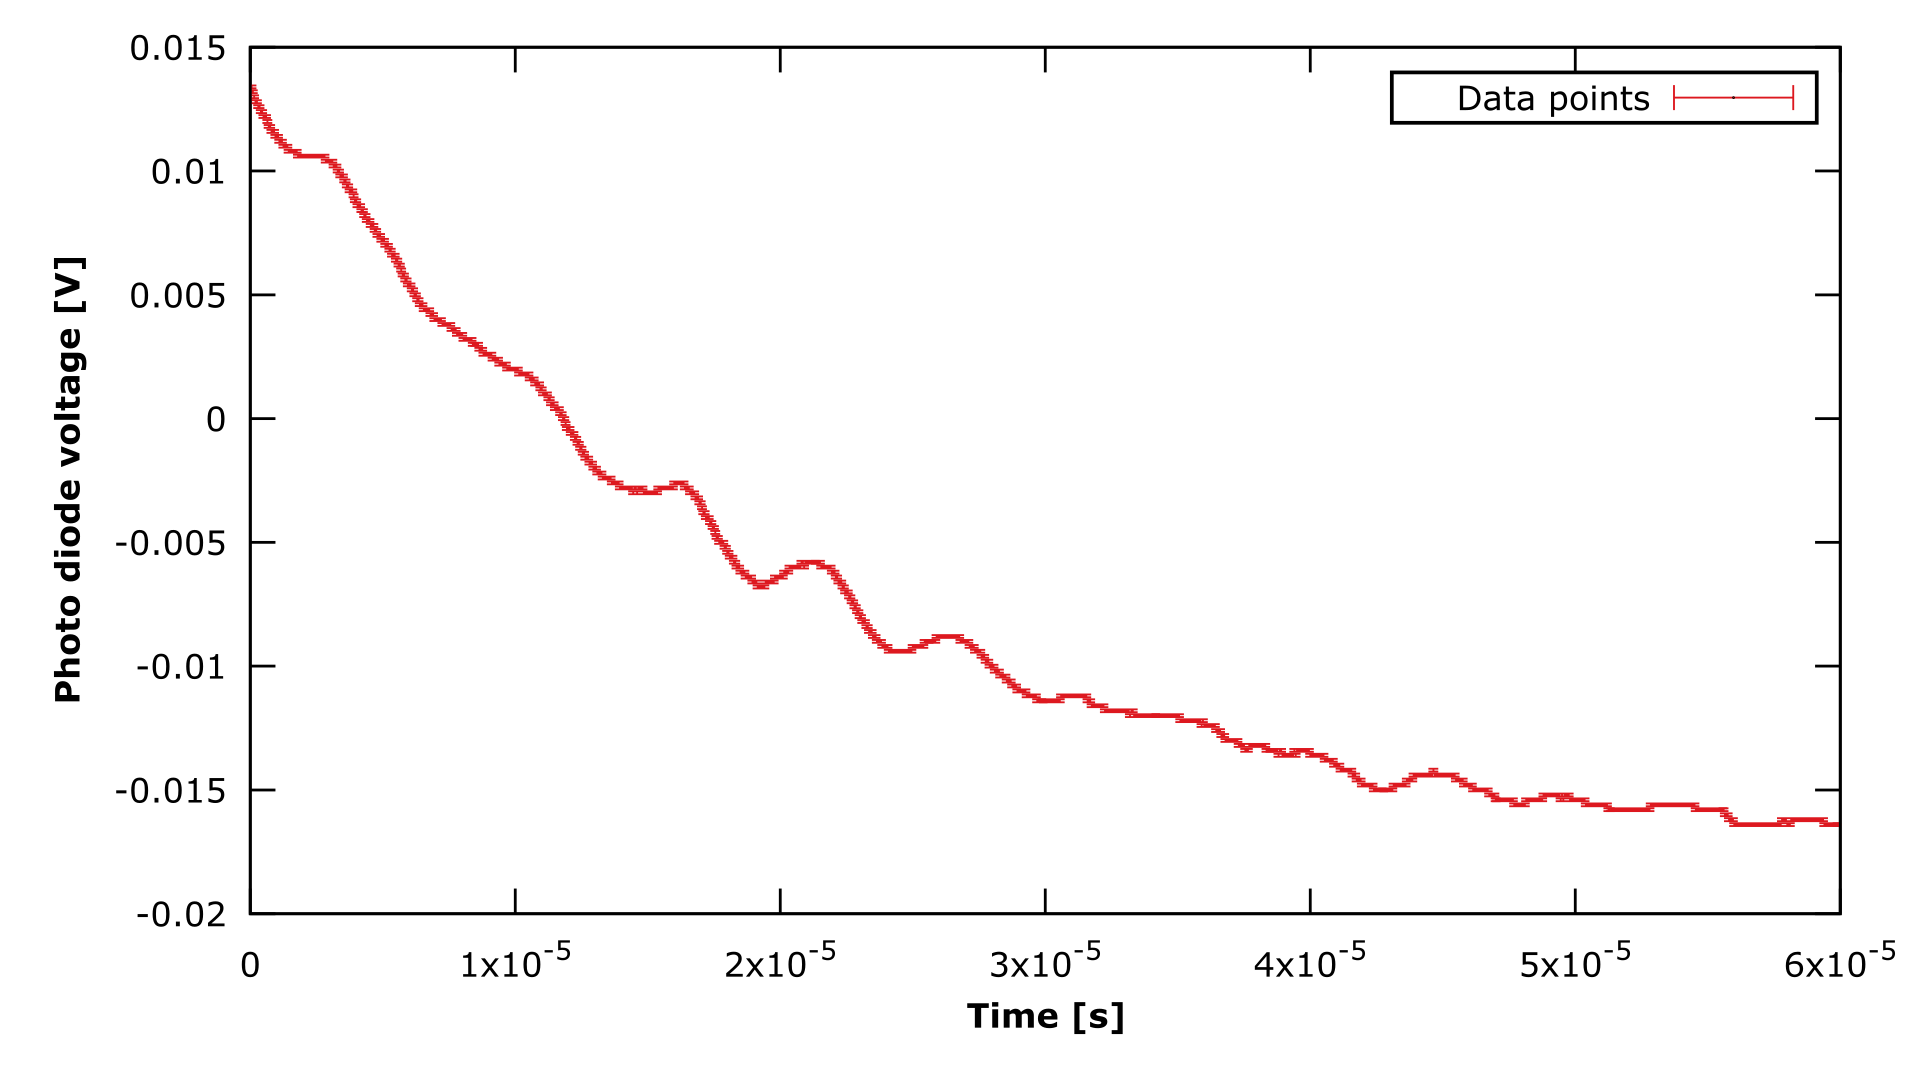
\includegraphics[width=1.0\linewidth]{graphics/spinprecessionexample}
	\caption[Example spin precession]{Examplary plot of the spin precession measurement. The peak positions were read off.}
	\label{fig:spinprecessionexample}
\end{figure}
Measurements were taken only for a diode current of $I_L=\unit{62.0}{mA}$, which was the current corresponding to $^{87}$Rb. No precession signal was found for $^{85}$Rb. The temperature during the measurements was $T=\unit{34.3}{\degree}$ and the current for the compensation of the horizontal field after turning the table was $I_{C1}=\unit{(6\pm1)}{mA}$.\\
The time differences between peaks were read out of appropriate sub plots of the recorded data. One exemplary plot can be seen in figure \ref{fig:spinprecessionexample} and all the values that were read out in table \ref{tb:precessionpeaks}. First, the time difference $\Delta t$ and its error were calculated
\begin{equation}
\Delta t=t_2-t_1, \qquad s_{\Delta t}=\sqrt{2}\cdot s_{t_{12}}
\end{equation}
where $s_{t_{12}}$ is the estimated error on reading the peaks as it is listed in table \ref{tb:precessionpeaks}.\\
There sometimes were no properly readable adjacent peaks. While it was always clear that there was a peak, it was much easier to read out the second most adjacent peak. Those values are marked with a star in the first column in table \ref{tb:precessionpeaks} and their time difference is
\begin{equation}
\Delta t=\frac{t_2-t_1}{2},\qquad s_{\Delta t}=\frac{1}{\sqrt{2}}s_{t_{12}}
\end{equation}
\newpage
The precession frequency $\nu_L$ can now be calculated
\begin{equation}
\nu_L=\frac{1}{\Delta t},\qquad s_{\nu_L}=\frac{s_{\Delta t}}{(\Delta t)^2}
\end{equation}
and the results are plotted in figure \ref{fig:freqlinfit}. A linear fit $f(x)=a\cdot x+b$ was used to describe the data and the resulting parameters were $a=\unit{(-3.40\pm0.17)}{kHz/mA}$ and $b=\unit{(280\pm11)}{kHz}$ with $\chi^2=9.9$. One can extrapolate to the magnetic field for which the precession frequency would be zero, assuming that all other fields were actually compensated for. The current in coil 4 for said field is $I^0_{C4}=\frac{-b}{a}=\unit{(82\pm5)}{mA}$ and the according magnetic field $B_v=\unit{39.2\pm2.5}{\micro T}$. This is within $1\sigma$ of the value calculated in the double resonance section.\\
Since the magnetic field is reduced until it reaches above field, the negative value of the fit constant $a$ corresponds to the proportionality constant $\alpha_{lit}=\unit{6.998}{kHz/\micro T}$ between the magnetic field and the precession frequency as it was defined in \ref{eq:precessionfreq}. It is however still given in kHz/mA and needs to be translated to kHz/\micro T to be comparable. The result is
\begin{equation}
\alpha=\frac{a}{c_b}\unit{(7.1\pm0.4)}{kHz/\micro T}
\end{equation}
where $c_b=\unit{0.476(1)}{\micro T/mA}$ is the proportionality factor between current and magnetic field for coil 4. This value includes the literature value in its $1\sigma$ interval.
\begin{table}
	\centering
	\begin{tabular}{@{}lllll@{}}
		\toprule
		&$I_{C4}$ [mA] &$\unit{t_1}{[10^{-5}s]}$ &$\unit{t_1}{[10^{-5}s]}$&$\unit{s_{t_{12}}}{[10^{-5}s]}$\\ 
		\midrule
		&0&2.0&2.5&0.1			\\
		&5&1.85&2.20&0.03		\\
		&10&2.01&2.42&0.03		\\
		&15&1.74&2.18&0.03		\\
		&20&1.93&2.42&0.03		\\
		&25&2.12&2.63&0.03		\\
		&30&1.80&2.38&0.03		\\
		&35&2.08&2.68&0.03		\\
		&40&4.25&5.00&0.03		\\
		&45*&4.52&5.32&0.04		\\
		&50*&5.37&7.23&0.04		\\
		&55*&5.38&7.23&0.05		\\
		&60*&4.74&7.10&0.06		\\
		&65*&5.45&8.03&0.08		\\
		&70*&14.4&17.8&0.12		\\
		&75&16.5&29.4&0.12		\\
		&80&15.0&20.2&0.13		\\
		&83&19.6&27.8&0.18		\\
		&90&21.9&27.8&0.45		\\
		\bottomrule
	\end{tabular}
	\caption[Properties of the magnetic field coils]{The $B/I$ values and properties of the Helmholtz coils. $n$ is the number of windings. \cite{anleitung}}
	\label{tb:precessionpeaks}
\end{table}
\begin{figure}
\centering
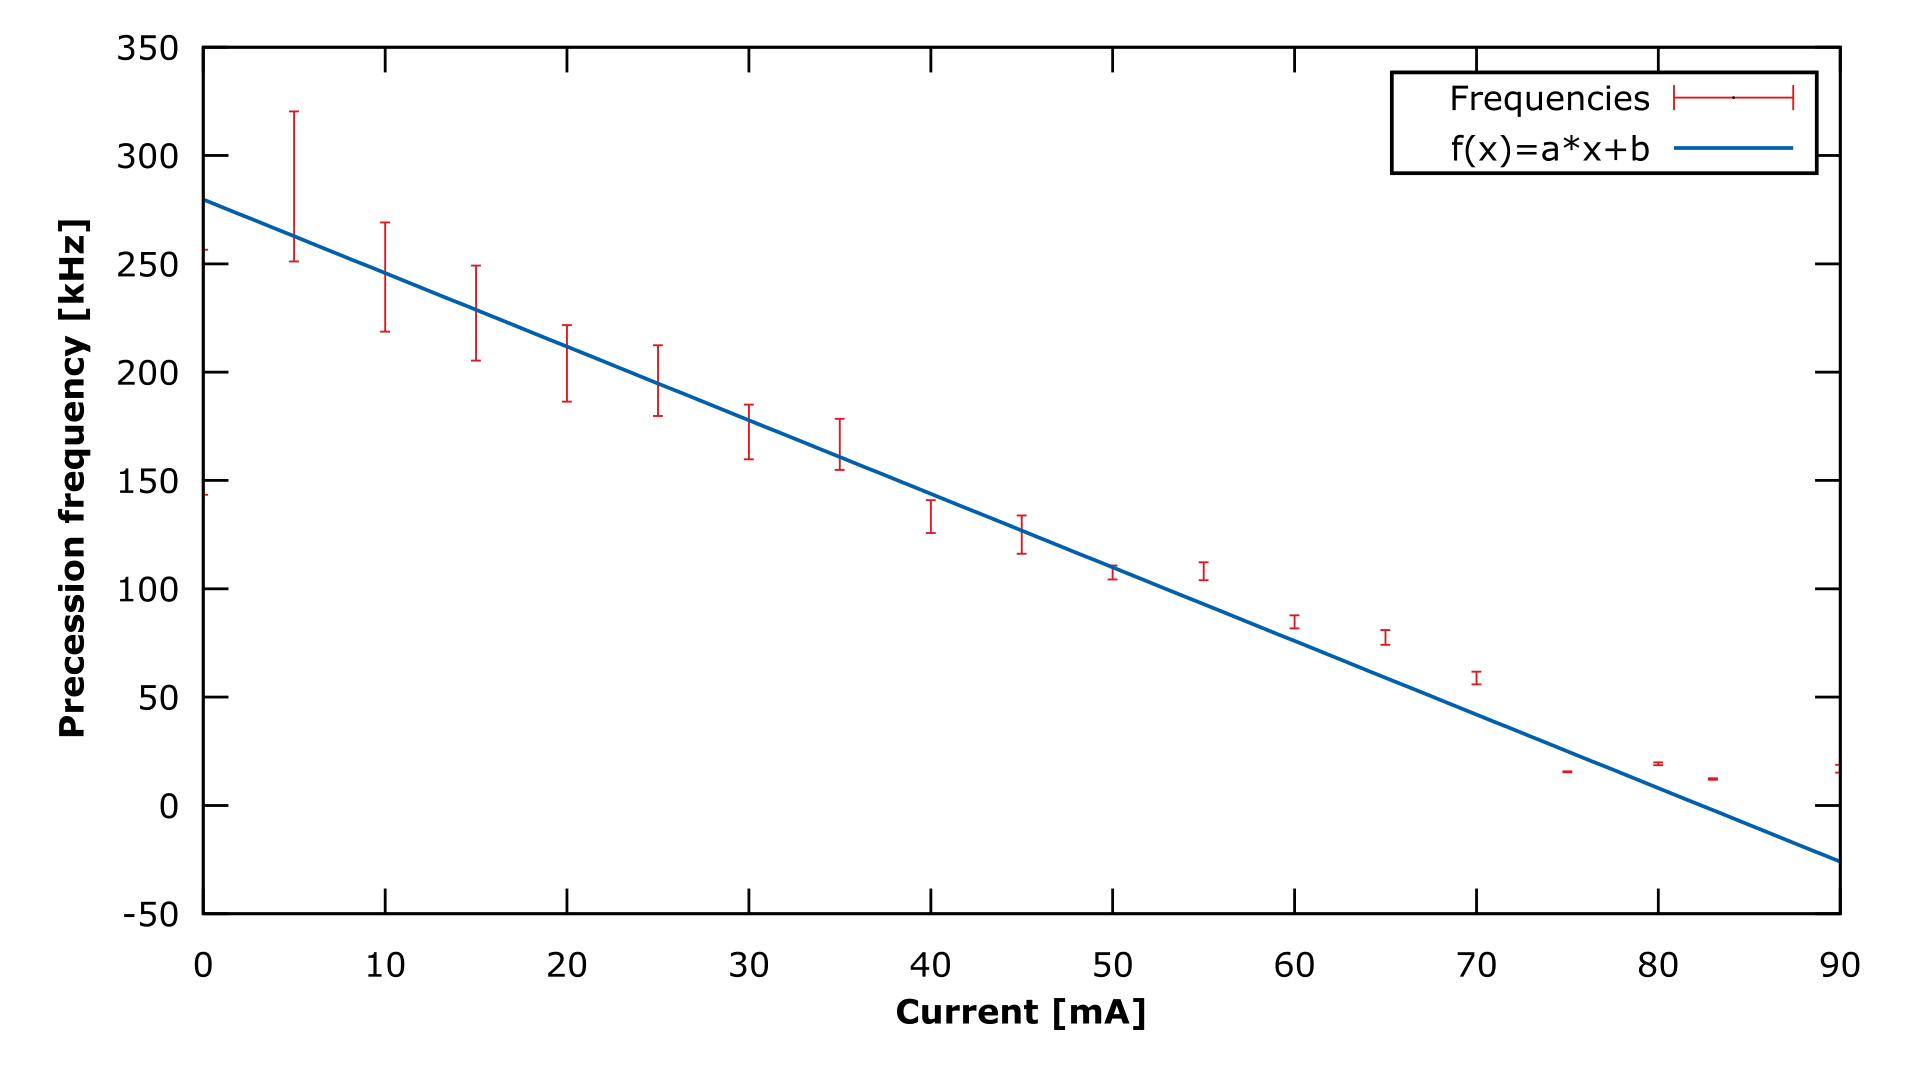
\includegraphics[width=1.0\linewidth]{graphics/freqlinfit}
\caption[Linear fit on precession frequencies]{The precession frequencies and the according linear fit. The x-axis cut can be calculated from the fit parameters and represents the current in coil 4 for which the vertical magnetic field is fully compensated.}
\label{fig:freqlinfit}
\end{figure}
